% Nallino, Part I p. 143: the image of the triquetrum, redrawn from the print: the upright FG, prolonged above F,
% standing in the base ABCD with its foot at G; the rule HM turning about the ring at H, marked at the 2nd to the
% 42nd of nearly equal steps from H (short strokes, every fifth longer and numbered 5 to 40, at the 30th the cross
% K), with the bar at its end M; the rule FL turning about the ring at F, its two sights traced from the print,
% and NF its prolongation. Measured on the scan (_intake/latin/tools/fig143).
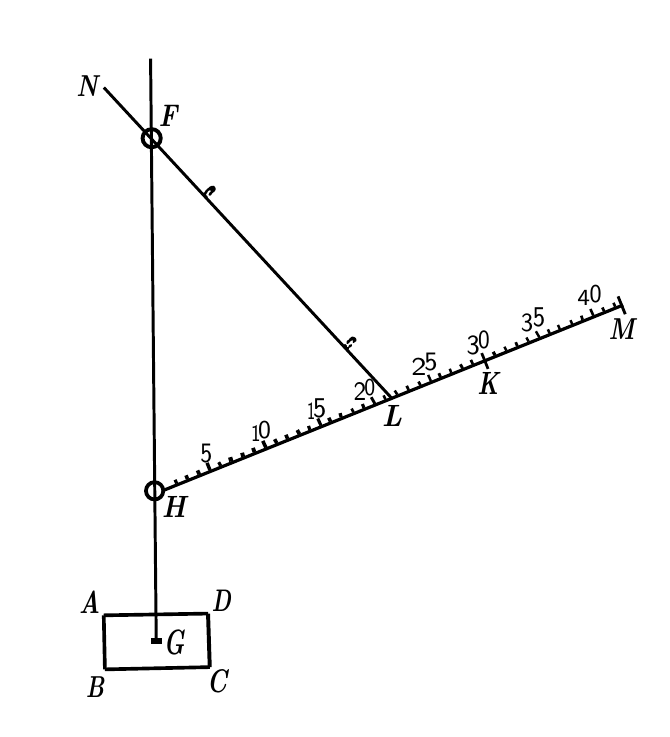
\begin{tikzpicture}[x=0.9928pt,y=-0.9928pt,line cap=butt,every node/.style={font=\fontsize{11}{11}\bfseries\itshape\selectfont,inner sep=0pt}]
\useasboundingbox (0,0) rectangle (223.50,248.00);
\draw[line width=1.40pt] (45.13,40.23) circle[radius=3.30];  % the ring at F
\draw[line width=1.36pt] (46.20,168.57) circle[radius=3.15];  % the ring at H
\draw[line width=1.07pt] (44.73,11.28) -- (46.79,223.20);  % the upright FG
\draw[line width=2.18pt] (44.96,223.20) -- (48.86,223.20);  % the foot of the upright at G
\draw[line width=1.16pt] (49.51,168.37) -- (216.75,100.94);  % the rule HM
\draw[line width=1.04pt] (217.50,104.29) -- (214.88,97.80);  % the bar at the end M
\draw[line width=0.99pt] (167.57,124.19) -- (165.25,118.44);  % the cross at 30 (K)
\draw[line width=1.06pt] (27.73,21.79) -- (132.53,134.89);  % the rule FL and its prolongation FN
\draw[line width=1.32pt] (27.69,213.89) -- (65.65,213.25);  % the base, side AD
\draw[line width=1.32pt] (28.11,233.56) -- (66.27,232.74);  % the base, side BC
\draw[line width=1.32pt] (27.69,213.89) -- (28.11,233.56);  % the base, side AB
\draw[line width=1.43pt] (65.65,213.25) -- (66.27,232.74);  % the base, side DC
\fill plot[smooth cycle,tension=0.5] coordinates {(65.06,62.07) (63.56,60.45) (63.70,60.35) (63.85,60.22) (64.00,60.08) (64.17,60.02) (64.34,59.94) (64.44,59.78) (64.54,59.62) (64.60,59.44) (64.74,59.30) (64.88,59.17) (65.02,59.03) (65.16,58.88) (65.28,58.73) (65.37,58.58) (65.53,58.50) (65.72,58.44) (65.86,58.31) (65.99,58.16) (66.06,57.99) (66.24,57.92) (66.41,57.85) (66.57,57.74) (66.73,57.66) (66.92,57.62) (67.12,57.62) (67.32,57.62) (67.48,57.52) (67.64,57.62) (67.84,57.62) (67.99,57.75) (68.05,57.93) (68.18,58.07) (68.28,58.23) (68.39,58.39) (68.40,58.58) (68.40,58.78) (68.40,58.98) (68.35,59.17) (68.21,59.30) (68.07,59.44) (68.02,59.63) (67.88,59.77) (67.73,59.89) (67.56,59.97) (67.42,60.11) (67.28,60.25) (67.14,60.38) (66.99,60.52) (66.94,60.70) (66.84,60.86) (66.72,60.98) (66.56,61.08) (66.36,61.10) (66.16,61.10) (65.99,61.03) (65.85,60.88) (65.82,60.74) (65.89,60.57) (66.00,60.41) (66.08,60.25) (66.14,60.06) (66.28,59.92) (66.46,59.86) (66.59,59.72) (66.60,59.52) (66.60,59.32) (66.50,59.18) (66.30,59.18) (66.12,59.24) (65.94,59.31) (65.80,59.44) (65.66,59.57) (65.52,59.72) (65.40,59.87) (65.39,60.07) (65.27,60.22) (65.13,60.36) (65.04,60.52) (64.93,60.67) (64.92,60.87) (65.03,61.03) (65.17,61.17) (65.35,61.23) (65.41,61.41) (65.52,61.56) (65.39,61.71) (65.25,61.85) (65.10,61.99)};  % a sight on FL, its printed outline
\fill plot[smooth cycle,tension=0.5] coordinates {(116.50,115.08) (116.30,115.10) (116.14,115.00) (116.05,114.84) (116.05,114.64) (116.05,114.44) (116.11,114.26) (116.18,114.09) (116.30,113.94) (116.44,113.80) (116.63,113.75) (116.77,113.61) (116.90,113.46) (117.04,113.32) (117.13,113.16) (117.24,113.01) (117.38,112.87) (117.56,112.81) (117.71,112.67) (117.87,112.58) (118.02,112.47) (118.22,112.46) (118.42,112.46) (118.59,112.54) (118.78,112.58) (118.94,112.66) (119.13,112.72) (119.27,112.85) (119.40,113.00) (119.46,113.18) (119.61,113.31) (119.65,113.50) (119.65,113.70) (119.65,113.90) (119.64,114.10) (119.45,114.16) (119.31,114.29) (119.17,114.43) (119.00,114.51) (118.85,114.62) (118.68,114.70) (118.49,114.75) (118.34,114.82) (118.33,114.62) (118.33,114.42) (118.33,114.22) (118.33,114.02) (118.31,113.82) (118.18,113.68) (118.03,113.78) (117.87,113.90) (117.71,113.99) (117.57,114.12) (117.38,114.18) (117.26,114.33) (117.19,114.50) (117.04,114.64) (116.90,114.78) (116.77,114.92) (116.59,114.99)};  % a sight on FL, its printed outline
\fill plot[smooth cycle,tension=0.5] coordinates {(116.86,117.00) (116.71,117.13) (116.56,117.27) (116.42,117.40) (116.28,117.35) (114.75,115.63) (114.90,115.50) (115.04,115.36) (115.19,115.23) (115.39,115.22) (115.59,115.22) (115.78,115.25) (115.92,115.39) (116.05,115.54) (116.12,115.71) (116.17,115.89) (116.17,116.09) (116.29,116.24) (116.47,116.30) (116.65,116.24) (116.77,116.09) (116.78,115.89) (116.89,115.74) (116.97,115.57) (117.11,115.43) (117.27,115.34) (117.47,115.34) (117.63,115.25) (117.82,115.22) (117.97,115.31) (117.97,115.51) (117.97,115.71) (117.95,115.91) (117.81,116.05) (117.66,116.18) (117.51,116.30) (117.35,116.39) (117.16,116.42) (116.99,116.51) (116.89,116.66) (116.89,116.86)};  % a sight on FL, its printed outline
% divisions of the rule HM, 0.90 pt wide
\draw[line width=0.89pt] (146.75,128.59)--(145.75,126.39) (154.16,125.60)--(153.63,124.14) (174.20,117.52)--(173.53,116.14) (182.31,114.25)--(181.54,112.77) (186.23,112.67)--(184.98,110.51) (193.69,109.67)--(192.99,108.22) (198.18,107.86)--(197.56,106.46);
% divisions of the rule HM, 0.95 pt wide
\draw[line width=0.94pt] (130.21,135.26)--(129.55,133.83) (134.52,133.52)--(133.60,132.08) (189.95,111.17)--(189.34,109.80) (205.87,104.76)--(204.82,102.39) (213.84,101.54)--(213.22,100.15);
% divisions of the rule HM, 1.00 pt wide
\draw[line width=0.99pt] (118.58,139.95)--(117.89,138.64) (138.66,131.85)--(137.95,130.36) (142.96,130.12)--(142.23,128.82) (162.02,122.44)--(161.30,120.93) (178.22,115.90)--(177.63,114.49) (201.98,106.32)--(201.49,104.82) (209.81,103.17)--(209.16,101.84);
% divisions of the rule HM, 1.05 pt wide
\draw[line width=1.04pt] (126.34,136.82)--(125.04,134.50) (150.26,127.18)--(149.66,125.77) (158.28,123.94)--(157.49,122.53);
% divisions of the rule HM, 1.15 pt wide
\draw[line width=1.14pt] (54.23,165.89)--(53.66,164.54) (70.25,159.43)--(69.52,158.16) (102.68,146.36)--(102.23,144.94) (106.71,144.74)--(105.60,142.26) (122.39,138.41)--(121.84,136.98) (170.09,119.18)--(169.41,117.98);
% divisions of the rule HM, 1.20 pt wide
\draw[line width=1.19pt] (114.09,141.76)--(113.70,140.29);
% divisions of the rule HM, 1.25 pt wide
\draw[line width=1.24pt] (66.34,161.01)--(65.30,158.41);
% divisions of the rule HM, 1.30 pt wide
\draw[line width=1.29pt] (58.18,164.30)--(57.63,162.92) (86.71,152.80)--(85.57,150.42) (90.66,151.20)--(89.89,149.79) (94.62,149.61)--(93.97,148.17) (110.24,143.31)--(109.58,141.98);
% divisions of the rule HM, 1.35 pt wide
\draw[line width=1.34pt] (62.47,162.57)--(61.81,161.14) (98.91,147.88)--(98.11,146.46);
% divisions of the rule HM, 1.40 pt wide
\draw[line width=1.39pt] (82.54,154.48)--(82.01,152.95);
% divisions of the rule HM, 1.45 pt wide
\draw[line width=1.44pt] (78.41,156.14)--(78.05,154.71);
% divisions of the rule HM, 1.55 pt wide
\draw[line width=1.54pt] (74.11,157.88)--(73.69,156.34);
\node at (21.62,21.20) {\normalfont\fontsize{11}{11}\bfseries\itshape\selectfont \resizebox{7.74pt}{7.51pt}{N}};
\node at (51.11,32.14) {\normalfont\fontsize{11}{11}\bfseries\itshape\selectfont \resizebox{6.77pt}{7.74pt}{F}};
\node at (53.22,174.28) {\normalfont\fontsize{11}{11}\bfseries\itshape\selectfont \resizebox{8.63pt}{7.62pt}{H}};
\node at (53.30,223.76) {\normalfont\fontsize{11}{11}\bfseries\itshape\selectfont \resizebox{7.58pt}{8.70pt}{G}};
\node at (22.49,209.16) {\normalfont\fontsize{11}{11}\bfseries\itshape\selectfont \resizebox{7.68pt}{7.86pt}{A}};
\node at (70.50,208.52) {\normalfont\fontsize{11}{11}\bfseries\itshape\selectfont \resizebox{6.99pt}{7.74pt}{D}};
\node at (24.56,239.84) {\normalfont\fontsize{11}{11}\bfseries\itshape\selectfont \resizebox{6.63pt}{7.51pt}{B}};
\node at (68.87,237.98) {\normalfont\fontsize{11}{11}\bfseries\itshape\selectfont \resizebox{7.31pt}{8.10pt}{C}};
\node at (167.58,129.34) {\normalfont\fontsize{11}{11}\bfseries\itshape\selectfont \resizebox{7.73pt}{7.98pt}{K}};
\node at (132.55,141.16) {\normalfont\fontsize{11}{11}\bfseries\itshape\selectfont \resizebox{7.29pt}{7.62pt}{L}};
\node at (216.15,109.62) {\normalfont\fontsize{11}{11}\bfseries\itshape\selectfont \resizebox{9.41pt}{7.51pt}{M}};
\node at (64.99,154.93) {\normalfont\fontsize{8}{8}\sffamily\selectfont \resizebox{4.32pt}{6.67pt}{5}};
\node at (83.02,147.80) {\normalfont\fontsize{8}{8}\sffamily\selectfont \resizebox{3.42pt}{5.60pt}{1}};
\node at (86.20,146.48) {\normalfont\fontsize{8}{8}\sffamily\selectfont \resizebox{4.64pt}{6.08pt}{0}};
\node at (103.17,139.52) {\normalfont\fontsize{8}{8}\sffamily\selectfont \resizebox{2.93pt}{5.84pt}{1}};
\node at (106.34,138.32) {\normalfont\fontsize{8}{8}\sffamily\selectfont \resizebox{4.78pt}{6.79pt}{5}};
\node at (120.97,132.57) {\normalfont\fontsize{8}{8}\sffamily\selectfont \resizebox{4.58pt}{6.31pt}{2}};
\node at (124.54,130.83) {\normalfont\fontsize{8}{8}\sffamily\selectfont \resizebox{3.92pt}{5.72pt}{0}};
\node at (142.43,123.58) {\normalfont\fontsize{8}{8}\sffamily\selectfont \resizebox{5.47pt}{6.08pt}{2}};
\node at (146.79,121.66) {\normalfont\fontsize{8}{8}\sffamily\selectfont \resizebox{4.78pt}{6.31pt}{5}};
\node at (162.18,115.55) {\normalfont\fontsize{8}{8}\sffamily\selectfont \resizebox{4.78pt}{6.55pt}{3}};
\node at (166.07,113.57) {\normalfont\fontsize{8}{8}\sffamily\selectfont \resizebox{4.21pt}{6.20pt}{0}};
\node at (181.75,107.34) {\normalfont\fontsize{8}{8}\sffamily\selectfont \resizebox{4.48pt}{6.20pt}{3}};
\node at (186.14,105.36) {\normalfont\fontsize{8}{8}\sffamily\selectfont \resizebox{4.48pt}{6.79pt}{5}};
\node at (202.41,98.28) {\normalfont\fontsize{8}{8}\sffamily\selectfont \resizebox{4.59pt}{5.48pt}{4}};
\node at (206.69,97.02) {\normalfont\fontsize{8}{8}\sffamily\selectfont \resizebox{4.35pt}{6.08pt}{0}};
\end{tikzpicture}
